% !TEX root = ../Диплом.tex

\section{Определения и понятия}

\subsection{Системы нелинейных ОДУ, полиномиальные и квадратичные системы}

В данной работе мы рассматриваем системы нелинейных ОДУ вида
\begin{equation} \label{eq:1}
    \begin{cases}
        \dot x_1 = f_1(\vec x)\\
        \vdots\\
        \dot x_n = f_n(\vec x)
    \end{cases},
\end{equation}
где $x_i$ - независимые переменные.

\begin{definition}
    Будем понимать под функциями $f_i(\vec x)$ нелинейные функции, которые могут быть записаны как линейные комбинации элементарных функций $g_k(\vec x)$. Назовём такие функции \textit{нелинейные функции с элементарными нелинейностями}.
    \begin{equation}
        f_i(\vec x) = p_i^T \vec x + a_{i,1} g_1(\vec x) + \cdots + a_{i,m} g_m(\vec x), p_i \in \mathbb{R}^n, a_j \in \mathbb{R}
    \end{equation}
\end{definition}



Таким образом, система \eqref{eq:1} может быть записана в матричной форме

\begin{equation}
    \frac{d}{dt} \vec x = P \vec x + Ag(\vec x)
\end{equation}

где $P^T = [p_1, \cdots, p_n], A = [a_ij], g(\vec x) = [g_1(\vec x), \cdots, g_m(\vec x)]$.

Заметим, что матрица $A$ может получиться крайне разреженной в силу того, что каждое дифференциальное уравнение обычно содержит лишь малую часть функций $g_j(\vec x) \in g(\vec x)$.

Так же, пользуясь тем, что комбинация элементарных функций является элементарной функцией, мы можем покрыть функциями $f$ широкий класс проблем, встречающихся на практике. Мы требуем элементарность функций, так как производная элементарной функции может быть найдена за конечное число шагов, что будет критично для нас в дальнейшем.

\begin{definition}
    Рассмотрим частный случай системы \ref{eq:1}, где функции $f_i$ представляют собой полиномы. Такие системы мы будем называть \textit{полиномиальными}.
\end{definition}

\begin{definition}
    Полиномиальная система имеет порядок $N$, если $N$ - наивысшая степень мономов, образованных переменными $x_i$.
\end{definition}

\begin{definition}
    Полиномиальные системы порядка 2 назовём \textit{квадратичными}
\end{definition}

\subsection{Методы полиномиализации} \label{poly-methods}

\begin{definition}
    Процесс преобразования нелинейных систем \ref{eq:1} к полиномиальному виду будем называть \textit{полиномиализацией}.
\end{definition}

\subsubsection{Полиномиализация с помощью введения алгебраических уравнений} \label{poly-algebraic}

Данный подход заключается в следующем алгоритме:
\begin{enumerate}
    \item Ввести новую переменную $y_i = g_i(\vec x)$, где $g_i(\vec x)$ - неполиномиальная нелинейная элементарная функция.
    \item Заменить $g_i(\vec x)$ на $y_i$ в оригинальном уравнении.
    \item  Добавить новое уравнение $y_i = g_i(\vec x)$ в систему.
\end{enumerate}

Как пример, рассмотрим уравнение $\dot x = x^3 + \frac{1}{1 + x}$. Тогда шаги алгоритма будут выглядеть следующим образом:
\begin{enumerate}
    \item Вводим новую переменную $y = \frac{1}{1 + x}$
    \item Делаем замену в первом уравнении $\dot x = x^3 + y$
    \item  Добавляем новое уравнение в систему $y = \frac{1}{1 + x}\; \Leftrightarrow \; xy + y - 1 = 0$
\end{enumerate}

Получили полиномиальную систему

$\begin{array}{lcl}
    \dot x = x^3 + y \\
    0 = xy + y - 1
\end{array}$
\newline

\begin{remark}
Важно заметить, что данный подход работает для ограниченного класса элементарных нелинейных функций, в частности для рациональных функций. Таким образом мы гарантируем полиномиальность вспомогательных уравнений. В том случае, если мы имеем дело со степенными функциями, логарифмами и многими другими элементарными нелинейностями, например $g_i(x) = e^x$, то получить полиномиальную систему данным методом мы уже не сможем.
\end{remark}


\subsubsection{Полиномиализация с помощью введения дифференциальных уравнений} \label{poly-diff}

Второй подход к полиномиализации предлагает добавление дифференциальных уравнений к системе.
Алгоритм похож на предыдущий за исключением последнего шага:

\begin{enumerate}
    \item Ввести новую переменную $_i = g_i(\vec x)$, где $g_i(\vec x)$ - неполиномиальная нелинейная элементарная функция.
    \item Заменить $g_i(\vec x)$ на $y_i$ в оригинальном уравнении.
    \item Добавить новое уравнение $\dot y_i = \dot g_i(\vec x) = g'_i(\vec x) \dot {\vec x}$ в систему. Данное уравнение получается как сложная производная от $g_i$.
\end{enumerate}
\newline

Таким образом, мы получим систему общего вида

\begin{equation}
    \begin{array}{lcl}
        \dot x_i = p_i^T \vec x + a_{i,1} y_1 + \cdots + a_{i,m} y_m,\quad i = 1, \cdots, n \\
        \dot y_i = \pounds_{\dot{\vec x}} g_i(\vec x) = g'_i(\vec x)(p_i^T \vec x + a_{i,1} y_1 + \cdots + a_{i,m} y_m,),\quad i = 1, \cdots, m
    \end{array},
\end{equation}
\newline
где $g'(\vec x) = \frac {dg(\vec x)}{d \vec x}$, $\pounds_{\dot{\vec x}}$ - производная Ли.

Так как $g'(\vec x)$ состоит только из полиномиальных функций от $x$ и $y_i$, данная система является полиномиальной.

\begin{example}
    Полиномиализуем уравнение $\dot x = sin(x)$. Тогда шаги алгоритма будут выглядеть следующим образом:
    \begin{enumerate}
        \item Избавляемся от $sin(x)$
        \begin{enumerate}
            \item Вводим новую переменную $y_1 =  sin(x)$
            \item Делаем замену в первом уравнении $\dot x = x^3 + y$
            \item Добавляем новое уравнение в систему $\dot y_1 = \dot {sin}(x) = cos(x) \dot x = sin(x) cos(x) = y_1 cos(x)$
            \item Получили систему $\begin{array}{lcl} \dot x = y_1\\ \dot y_1 = y_1 cos(x) \end{array}$
        \end{enumerate}
        \item Избавляемся от $cos(x)$
        \begin{enumerate}
            \item Вводим новую переменную $y_2 =  cos(x)$
            \item Делаем замену во втором уравнении $\dot y_1 = y_1 y_2$
            \item Добавляем новое уравнение в систему $\dot y_2 = \dot {cos}(x) = -sin(x) \dot x = -y_1^2$
        \end{enumerate}
    \end{enumerate}
    
    Получили полиномиальную систему
    
    $\begin{array}{lcl}
        \dot x = y_1\\
        \dot y_1 = y_1 y_2\\
        \dot y_2 = -y_1^2
    \end{array}$
\end{example}



\begin{theorem}
    \begin{enumerate}
    \item Итеративно применяя алгоритмы полиномиализации с помощью введения алгебраических и дифференциальных уравнений, нелинейную систему с элементарными нелинейностями можно привести к полиномиальной форме.
    \item Размер полученной полиномиальной системы является линейным относительно числа элементарных функций в     оригинальной системе.
\end{enumerate}
\end{theorem}

\begin{proof}
    Доказательство первой части уже изложено вместе с алгоритмами полиномиализации.
    
    Рассмотрим вторую часть.
    Заметим, что для того, чтобы избавиться от основной (не композитной) элементарной функции,
    требуется конечное число замен $O(1)$, обычно 1 или 2, например для $sin(x)$.
    
    Для композитных элементарных функций $g(\vec x) = (g_1 \circ g_2 ... \circ g_n)(\vec x)$ необходимо потратить $O(1 \cdot m)$ замен.
    Таким образом, размер полученной полиномиальной системы линеен относительно числа элементарных функций в оригинальной системе.
\end{proof}


\subsection{Методы квадратизации}

\begin{definition}
    Процесс преобразования нелинейных систем \ref{eq:1} к квадратичному виду будем называть \textit{квадратизацией}.
\end{definition}

В данном разделе мы будем рассматривать квадратизации только полиномиальных систем, которые мы уже умеем получать с помощью полиномиализации из систем \ref{eq:1}. Так же заметим, что подходы, применяемые для квадратизации систем, весьма похожи на методы полиномиализации.

\subsubsection{Квадратизация с помощью введения алгебраических уравнений}

Данный подход заключается в следующем алгоритме

\begin{enumerate}
    \item Ввести новую переменную $y_i = m_i(\vec x)$, где $m_i(\vec x) = x_1^{b_1}\cdot \cdots \cdot x_n^{b_n}$ - моном, образованный из переменных системы.
    \item Заменить $m_i(\vec x)$ на $y_i$ в оригинальном уравнении.
    \item Добавить новое уравнение $y_i = m_i(\vec x)$ в систему.
\end{enumerate}

\begin{example}
    Квадратизуем систему, полученную в примере раздела \ref{poly-algebraic}

    $\begin{array}{lcl}
        \dot x = x^3 + y_1 \\
        0 = xy_1 + y_1 - 1
    \end{array}$
    \newline
    
    Теперь проведём квадратизацию
    
    \begin{enumerate}
    	\item Вводим новую переменную $y_2 =  x^2$
    	\item Делаем замену в первом уравнении $\dot x = xy_2 + y_1$
    	\item Добавляем новое уравнение в систему $y_2 - x^2 = 0$
    \end{enumerate}
    
    Получили квадратичную систему
    
    $\begin{array}{lcl}
        \dot x = xy_2 + y_1 \\
        0 = xy_1 + y_1 - 1 \\
        0 = y_2 - x^2
    \end{array}$
\end{example}


\subsubsection{Квадратизация с помощью введения дифференциальных уравнений}

Данный подход заключается в следующем алгоритме:
\begin{enumerate}
    \item Ввести новую переменную $y_i = m_i(\vec x)$, где $m_i(\vec x) = x_1^{b_1}\cdot \cdots \cdot x_n^{b_n}$ - моном, образованный из переменных системы.
    \item Заменить $m_i(\vec x)$ на $y_i$ в оригинальном уравнении
    \item Добавить новое уравнение $\dot y_i = \dot {m_i}(\vec x) = m'_i(\vec x) \dot{\vec x}$ в систему, где $m'(\vec x) = \frac {dm(\vec x)}{d \vec x}$
\end{enumerate}

\begin{example}
    Рассмотрим систему

    $\begin{array}{lcl}
        \dot x = xz^2 + z \\
        \dot z = x \\
    \end{array}$
    \newline
    
    Теперь проведём квадратизацию:
    \begin{enumerate}
        \item Вводим новую переменную $y = z^2$
        \item Делаем замену в первом уравнении $\dot x = xy + z$
        \item Добавляем новое уравнение в систему $\dot y = 2z \dot z = 2xz$
    \end{enumerate}
    
     Получили квадратичную систему
    
    $\begin{array}{lcl}
        \dot x = xy + z \\
        \dot y = 2xz \\
        \dot z = x \\
    \end{array}$
\end{example}


\subsection{Абстрактные синтаксические деревья} \label{AST-section}

Для того, чтобы удобно работать с математическими выражениями, нам понадобится определить на них структуру.
Для этого мы воспользуемся синтаксическим анализом - процессом преобразования последовательности лексем формального языка с его формальной грамматикой.
Результатом обычно является дерево разбора, которое отражает синтаксическую структуру входной последовательности лексем.

В нашем случае мы получаем на вход строковое представление математического выражения, а возвращаем дерево разбора, состоящее из внутренних узлов, представляющий математические функции, например как сложение или взятие логарифма, и листьев, состоящих из переменных и чисел.

\begin{figure}[h!]
    \centering
    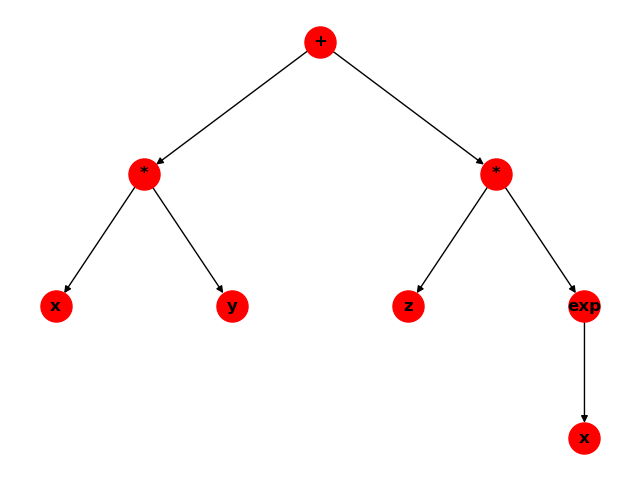
\includegraphics{chapters/images/AST.png}
    \caption{Абстрактное синтаксическое дерево выражения $x \cdot y + z \cdot exp(x)$}
    \label{fig:AST}
\end{figure}

Абстрактное синтаксическое дерево (\textit{АСД}, \textit{AST}) отличается от дерева разбора тем, что в нём отсутствуют узла и рёбра, которые не влияют на семантические свойств выражения. Например, для выражения $3 + 2 \cdot 4$ не нужно расставлять группирующие скобки, так как приоритет операции умножения задан выше, чем приоритет операции сложения.

Многие языки программирования и системы компьютерной алгебры используют данный подход для обработки для обработки своих выражений. В частности, АСД использует фреймворк SymPy \cite{SymPy}, реализованный на языках программирования Python и Julia, который мы будем использовать в дальнейшем.

Оба подхода к полиномиализации, приведённые в пункте \ref{poly-methods}, на первом шаге требуют найти какую-нибудь элементарную нелинейную функцию. Пользуясь средствами синтаксического анализа, мы можем представить правые части системы \ref{eq:1} как абстрактные синтаксические деревья. Таким образом, мы можем свести задачу поиска нужной элементарной функции к задаче поиска на графе. Подробное решение данной задаче находится в пункте \ref{poly-algo}.

\subsection{Граф замен} \label{replacement-graph-section}

Как в процессе полиномиализации, так и в процессе квадратизации, на каждом шаге итерации алгоримта мы выбираем следующую замену переменной. Данный шаг можно обобщить следующим образом.

Граф замен - ацикличный ориентированный граф, чьи вершины представляют системы уравнений, эквивалентные заданной системе, а дуги - преобразования, совершаемые с помощью замены переменной. Входной вершиной мы полагаем заданную систему, а выходной - систему, обладающей нужными нам свойствами.

\begin{wrapfigure}{l}{11cm}
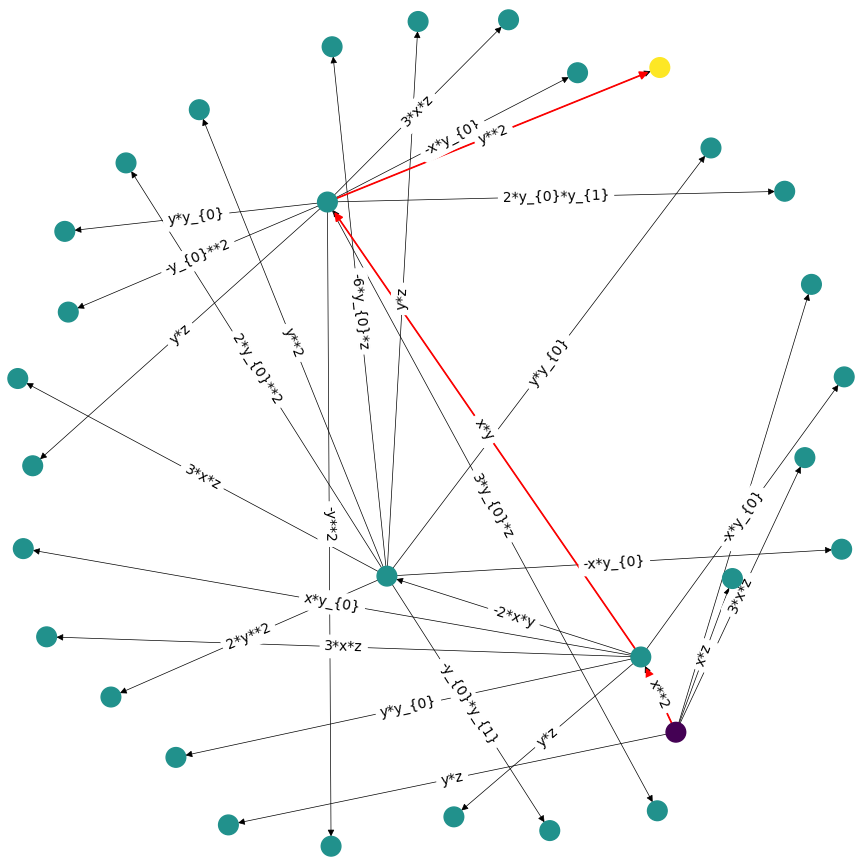
\includegraphics[width=10.5cm,height=10.5cm]{chapters/images/replacement_graph.png} 
\caption{Граф замен}
\label{fig:replacement-graph}
\end{wrapfigure}

Таким образом, мы можем трактовать задачу об оптимальном преобразовании как задачу поиска путей на графе с одним входом и несколькими выходами. Важно заметить, что графы замен, которые нам будут встречаться на практике, часто являются огромными и заранее задан только начальный узел.

В силу того, что квадратизация является гораздо более требовательной к заменам \cite{Gu-PhD}, мы не сможем выбирать замены в произвольном порядке и быстро достичь при этом квадратичной системы. Поэтому мы будет пользоваться алгоритмами поиска на графе замен, что описано в секции \ref{quad-algo}

\subsection{Алгоритмы поиска на графе} \label{search-algo}

В данном разделе мы рассмотрим основные алгоритмы поиска на графе. Подчеркнём, что сам путь нас не интересует, поэтому мы приводим алгоритмы поиска пути на графах, которые, в связи с этим упрощаются.

Пусть $G$ - ориентированный граф, $V$ - множество его рёбер, $E$ - множество его дуг.

\subsubsection{Поиск в глубину (DFS)} \label{DFS-algo}

Поиск в глубину (depth-first search, DFS) заключается в том, что, начиная со стартового узла, исследует его ветви как можно дальше, далее переходя к исследованию других ветвей. Несмотря на то, поиск в глубину применяется в основном при анализе достижимости, он, тем не менее, может находить путь из одной вершины в другую, пусть и не гарантируется то, что найденный путь будет кратчайшим.

\begin{algorithm}[H]
\SetAlgoLined
\SetKwFunction{FDFS}{DFS}
\SetKwProg{Fn}{Function}{:}{}
\KwData{G - входной граф \\
    prop - свойство, которым должна обладать выходная вершина \\
    visited - массив, хранящий для каждой вершины бит, показывающий, посещали ли мы эту вершину}
\KwResult{Вершина, обладающая свойством prop или null, если вершина не найдена}

\Fn{\FDFS{G, v, prop}}{
    visited[v] = true\;
    \If{v обладает свойством prop}{
        \Return v\;
    }
    \ForEach{w: сосед v}{
        \If{visited[w] == false}{
            \Return \FDFS(G, w, prop)\;
        }
    }
    \Return null\;
}
\caption{Поиск в глубину}
\label{algo:DFS}
\end{algorithm}

В худшем случае DFS найдёт искомую вершину последней, поэтому худшая оценка числа операций:
\begin{enumerate}
    \item Чтобы пометить каждую вершину в начале мы посещаем ровно $|V|$ вершин.
    \item В худшем случае мы пройдём по всем дугам графа $|E|$.
\end{enumerate}

Таким образом, число операций в худшем случае можно оценить как $O(|V| + |E|)$

Среднее время работы уже зависит от \textit{prop}.

\subsubsection{Поиск в ширину (BFS)} \label{BFS-algo}

В поиске в ширину (breadth-first search, BFS) граф разбивается на слои: сама входная вершина, вершины на расстоянии 1 от входной вершины, вершины на расстоянии 2 и так далее. Сам поиск исследует слои по возрастанию глубины, пока не найдёт искомую вершину. В отличие от поиска в глубину, BFS всегда отыскивает кратчайший путь до неё.

\begin{algorithm}[H]
\SetAlgoLined
\SetKwFunction{FBFS}{BFS}
\SetKwProg{Fn}{Function}{:}{}
\KwData{G - входной граф \\
    prop - свойство, которым должна обладать выходная вершина \\
    visited - массив, хранящий для каждой вершины бит, показывающий, посещали ли мы эту вершину}
\KwResult{Вершина, обладающая свойством prop или null, если вершина не найдена}

\Fn{\FBFS{G, v_{start}, prop}}{
    \tcc{Очередь из одного элемента}
    Q = \{v_{start}\}\;
    \While{Q не пуста}{
        v = Вытолкнуть(Q)\;
        visited[v] = true\;
        \If{v обладает свойством prop}{
            \Return v\;
        }
        \ForEach{w: сосед v}{
            \If{visited[w] == false}{
                Вставить(Q, w)\;
            }
        }
     }
     \Return null\;
 }
\caption{Поиск в ширину} \label{algo:BFS}
\end{algorithm}

Оценим время работы алгоритма в худшем случае.
\begin{enumerate}
    \item Мы посещаем каждую вершину дважды: в том время, когда мы её помещаем, и при вставке её в очередь: $2|V|$
    \item Каждое ребро в фунции BFS просматривается ровно 1 раз: $|E|$
\end{enumerate}

Таким образом получим оценку $O(|V| + |E|)$, как и у поиска в глубину.

Так же, можно получить альтернативную оценку как числа шагов, так и пространственную сложность в виде $O(b^{d})$, где $b$ - средний коэффициент ветвления графа, $d$- глубина на которой находится выходная вершина. Пусть мы обычно и не знаем $b$ и $d$ точно, но, зная их примерные оценки, мы можем пользоваться данным методом оценки для заранее неисследованных графов.

\subsubsection{Поиск с ограничением глубины (DLS)} \label{DLS-algo}

Поиск с ограничением глубины (depth-limited search, DLS) - вариант поиска в глубину, для которого определяется конечная глубина l на которую он может опуститься. Таким образом, алгоритм всегда работает конечное число шагов, в отличие от DFS, однако ответ не может быть найден, если глубина выходного узла d > l.

\begin{algorithm}[H]
\SetAlgoLined
\SetKwFunction{FDLS}{DLS}
\SetKwProg{Fn}{Function}{:}{}
\KwData{G - входной граф \\
    prop - свойство, которым должна обладать выходная вершина \\
    visited - массив, хранящий для каждой вершины бит, показывающий, посещали ли мы эту вершину \\
    l - предельная глубина}
\KwResult{Вершина, обладающая свойством prop или null, если вершина не найдена}

\Fn{\FDLS{G, v, prop, depth, l}}{
    visited[v] = true\;
    \If{v обладает свойством prop}{
        \Return v\;
    }
    \ForEach{w: сосед v}{
        \If{visited[w] == false \& depth < l}{
            \Return \FDFS(G, w, prop, depth + 1, l)\;
        }
    }
    \Return null\;
}
\caption{Поиск с ограничением глубины} 
\label{algo:DLS}
\end{algorithm}

В худшем случае, число шагов алгоритма оценивается как $O(b^l)$, а пространственная сложность как $O(b \cdot l)$. Таким образом, мы получили лучшие оценки, чем для BFS, при условии, что конечная l выбрана правильно. Гарантировать это поможет следующий алгоритм.

\subsubsection{Поиск в глубину с итеративным углублением (ID-DFS)} \label{ID-DFS-algo}

Поиск в глубину с итеративным углублением (iterative-deepening depth-first search, ID-DFS) запускает DLS на каждой своей итерации и, в случае неудачи, увеличивает конечную глубину l.

\begin{algorithm}[H]
\SetAlgoLined
\SetKwFunction{FIDDFS}{IDDFS}
\SetKwFunction{FDLS}{DLS}
\SetKwProg{Fn}{Function}{:}{}
\SetKwRepeat{Do}{do}{while}
\KwData{G - входной граф \\
prop - свойство, которым должна обладать выходная вершина}
\KwResult{Вершина, обладающая свойством prop или null, если вершина не найдена}

 \Fn{\FIDDFS{G, v_{start}, prop}}{
    l = 1\;
    
    \Do{v == null}{
        v = \FDLS{G, v, prop, 1, l}\;
        l += 1\;
    }
    \Return v\;
 }
\caption{Поиск в глубину с итеративным углублением}
\label{algo:ID-DFS}
\end{algorithm}

Оценкой сложности алгоритма является $O(b^d)$ как у поиска в ширину, а пространственная сложность представляет $O(b \cdot d)$ как у поиска с ограничением глубины, что позволяет ID-DFS использовать преимущества обоих походов.

\subsubsection{Эвристический подход к поиску}

Эвристический поиск, он же информированный поиск представляет собой семейство стратегий поиска,
в котором используются знания о конкретной задаче, зачастую позволяя решать задачу поиска гораздо эффективнее.

Знания о задаче формализуются в качестве эвристических функций.
Эвристические функции сравнивают между собой варианты, из которых алгоритм выбирает следующий шаг.

В случае задач поиска на графе, с помощью эвристических функций мы будем сортировать дуги алгоритмов неинформативного поиска.

Приведём эвристические версии алгоритмов неинформативного поиска
\begin{enumerate}
    \item DFS $\rightarrow$ Поиск по первому наилучшему совпадению (best-first search)
    \item Алгоритм Дейкстры $\rightarrow$ Алгоритм A*
    \item ID-DFS $\rightarrow$ Алгоритм А* с итеративным углублением (Iterative deepening A*, IDA*)
\end{enumerate}


Эвристики, которыми мы будем пользоваться для задачи квадратизации, подробно описаны в секции \ref{heuristics}